
\section{Introduction} 
\label{sec:introduction}
	
	This machine learning master thesis is about neural networks (section \ref{sec:neural_networks}). 


	\subsection{Motivation}
		At the very beginning of this thesis, there is me, the writer. I wanted, from the very first day, to work on neural-networks and more specifically on deep-learning. I wanted so, because deep-learning has become in the last decade the most efficient algorithm at classifying images. 
		I was then searching for a topic and discovered the work made by Ian J. Goodfellow, Jonathon Shlens and Christian Szegedy. In their publication named "Explaining and Harnessing Adversarial Examples"\cite{goodfellow2014explaining} they motivate that adversarial learning could improve the accuracy of some given neural-networks. Most of their test are based on the MNIST dataset\cite{lecun-mnist}. After contacting one of the authors of this publication, it appeared that it would be a good contribution to validate their observations on other datasets. For this reason, the following thesis is about validating the proposed adversarial learning described in \cite{goodfellow2014explaining} with different datasets.

	\subsection{Methodology}
		On the one hand , we want to validate that adversarial learning is performing better at classifying than regular learning. On the other hand, we  want to understand the reasons underlining this performances. To do so, we will first re-implement the proposed solution of \cite{goodfellow2014explaining} in such way that we isolate adversarial learning from other techniques used in the paper. Once this is done, we will move to other datasets. These datasets are composed 

		step we will take is to re-implement adversarial learning on the MNIST dataset. This operation will 
		Once we have implemented the neural networks and trained the dataset with this adversarial learning technique, we expect to have a model more accurate in predicting the classes. 
		It seems legitimate at this point to believe that adversarial learning will improve the accuracy of predicting images' classes. The paper presented above\cite{goodfellow2014explaining} was classifying a dataset composed by images: the MNIST dataset. What we are going to do in this paper is to first validate this hypothesis with another image dataset: the CIFAR10 dataset\cite{krizhevsky2009learning} and the STL-10 dataset\cite{maybe...}. Once the hypothesis is more accepted, we would like to try this technique on a dataset of other nature. The one we would try is a phoneme dataset: the TIMIT dataset\cite{maybe...}. Having better results with these datasets would further validate this technique as useful for classification in the context of shallow neural network.

	\subsection{Expected outcome}
	
	In their paper, Ian J. Goodfellow, Jonathon Shlens and Christian Szegedy, described their technique to able to ??? 
	=> How adversarial learning best separate the classes.




	\subsection{Setting-up an example}
		To understand our adversarial training we will use a simple neural network composed by two sigmoid neurons (see section \ref{sec:Artificial_neurons}). The network aims a recognizing a columns and a dot in a three by one pixels image. This network is sketched on \fref{fig:2N_NN}. Considering a white pixel has value $1$ and a dark pixel has value $0$, a column could be represented by a vector $x^1 = [1,0,1]$ and a dot could be by $x^2 = [0,0,1]$. We consider the column to be the output $y^i = 0$ and the dot to be the output $y^i = 1$
		To predict a sensible value, a two-sigmoid network could use the weights and biases :
		$$ W = \left( \begin{matrix} 1 & -1 \\ -1 & -1 \\ 1 & 1 \end{matrix} \right) ; b = \left( \begin{matrix} -1.5 & 0.5 \end{matrix} \right)$$
		
		\vskip 1em
		\textbf{signal propagation: } The input signal $x^i$ propagates through the network resulting in a prediction vector $p^i = \sigma(W^Tx + b)$. To know how right or wrong is this prediction vector, we would use a cost function like the negative log-likelihood:
		$$ C^i = y^i \ln(p^i) + (1-y^i)\ln(1-p^i) $$
		Propagating $x^1$ and $x^2$, we get that $p^1 = [\sigma(.5), \sigma(-.5)]$ and $p^2 = [\sigma(-.5), \sigma(.5)]$

		\begin{figure}
			\centering
			\def\layersep{1.5cm}	
			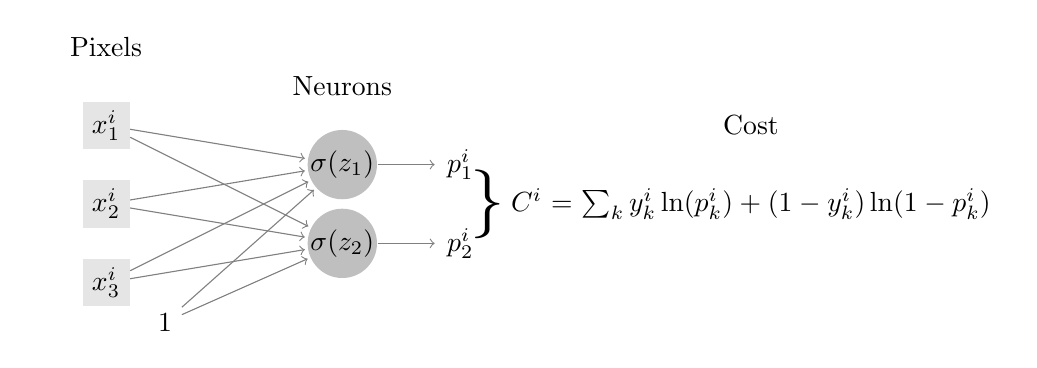
\begin{tikzpicture}[shorten >=1pt,->,draw=black!50, node distance=\layersep]
			    \tikzstyle{every pin edge}=[<-,shorten <=1pt]
			    \tikzstyle{pixel} = [rectangle, fill=black!10,minimum size=17pt,inner sep=0pt]
			    \tikzstyle{neuron}=[circle,fill=black!25,minimum size=17pt,inner sep=0pt]
			    \tikzstyle{annot} = [text width=5em, text centered]
			    \tikzstyle{annot2} = [text width=18em, text centered]
				\tikzstyle{accolade} = [rectangle, text centered, minimum size=17pt]
			    
			    %%% DRAW THE NODES
			    \foreach \name / \y in {1,2,3}
			        \node[pixel] (I-\name) at (0,-\y) {$x^i_\y$};
			    \node[] (I-4) at (\layersep/2,-3.5) {$1$};
			    \foreach \name / \y in {1,2}
					\node[neuron] (O-\y) at (\layersep*2,-\y-0.5) {$\sigma(z_\y)$};
				\foreach \name / \y in {1,2}	
					\node[] (C-\y) at (\layersep*3,-\y-0.5) {$p^i_\y$};

			    %%% DRAW THE PATHS
			    \foreach \source in {1,...,4}
			        \foreach \dest in {1,2}
			            \path (I-\source) edge (O-\dest);
			    \foreach \y in {1,2}
			        \path (O-\y) edge (C-\y);

			    %%% ANOTATE
			    \node[accolade] at (\layersep*3+1em,-2) { \Huge\} };
			    \node[annot2] at (\layersep*3+10.5em,-2) (cost) {$C^i = \sum_k y^i_k \ln(p^i_k) + (1-y^i_k)\ln(1-p^i_k) $};

			    \node[annot,above of=I-1, node distance=1cm] (iv) {Pixels};
			    \node[annot,above of=O-1, node distance=1cm] (iv) {Neurons};
			    \node[annot,above of=cost, node distance=1cm] (iv) {Cost};

			\end{tikzpicture}
			\label{fig:2N_NN}
			\caption{Two neurons neural network}
		\end{figure}


	\subsection{Adversarial learning}
		Imagine you are allowed to modify each pixels of our image by a value $\epsilon$. Intuitively, if you want to improve the recognition, you would increase the contrast in the picture and insist on the dots where the aught to be. On the other hand, if you want to confuse the recognition, you would lower the contrast and add color where there shouldn't be.

		These properties are the ones we aught to enforce with our adversarial learning. For an epsilon small enough, we subtract to $x^i$ $\epsilon$ times the sign of the derivative with respect to $x^i$ of the Cost $C^i$.
		$$ x^{i_{\text{adv}}} \leftarrow x^i - \epsilon \text{ sign}(\nabla_{x^i} C^i) $$
		Therefore the input $x^i$ is modified such that ?? TODO: HERE IS THE THING ??

		\vskip 1em
		\textbf{In our example. } We apply the adversarial learning to our example. First we compute the derivative of the Cost with respect to $x^i$. (The mathematics behind this derivative is detailed on the appendix \ref{sec:2N_NN_cost})
		$$	\frac{\delta C^i}{\delta x^i} = W \cdot \left( y^i -p^i \right) $$
		Then we subtract the sign of this derivative to the actual input $x^i$
		\begin{equation}
			\begin{split}
				x^{1_{\text{adv}}} &\leftarrow x^1 - \epsilon \text{ sign}(\nabla_{x^1} C(W,b,x^1)) \\
				x^{1_{\text{adv}}} &\leftarrow x^1 - \epsilon \text{ sign}( W \cdot ( y^i -p^i) )
			\end{split}
		\end{equation}
		\begin{equation}
			x^1 = \left( \begin{matrix} 1 \\ 0 \\ 1 \end{matrix} \right) ;
			x^{1_{\text{adv}}} = \left( \begin{matrix} .7 \\ 0 \\ 1 \end{matrix} \right) ;
			x^2 = \left( \begin{matrix} 0 \\ 0 \\ 1 \end{matrix} \right) ;
			x^{2_{\text{adv}}} = \left( \begin{matrix} .3 \\ 0 \\ 1 \end{matrix} \right) ;
		\end{equation}
		


		Once we have these derivatives, the worst modification we can make to sample $x^i$ is by following this derivative. 
		

	\subsection{Dataset}
		The first dataset we will be using is the MNIST\ref{??} dataset. This dataset is composed by 60k gray scale images. Each of them represent a hand written digit (6k of each). 







		